\documentclass[11pt,a4paper]{article}
\usepackage[a4paper,margin=23mm]{geometry}
\usepackage[T1]{fontenc}
\usepackage{tgpagella}
\usepackage{tgheros}
\usepackage[scaled=0.80]{DejaVuSansMono}
\usepackage{microtype}
\usepackage{graphicx}
\usepackage{amsmath}
\usepackage{xcolor}
\usepackage{listings}
\usepackage{caption}
\usepackage{float}
\usepackage{booktabs}
\usepackage{tabularx}
\usepackage{pdfpages}
\usepackage{tikz}
\usepackage{titlesec}
\usepackage[colorlinks=true,linkcolor=blue!45!black,urlcolor=blue!55!black]{hyperref}
\pdfminorversion=7

\definecolor{navy}{HTML}{173B57}
\definecolor{blue}{HTML}{2F6F9F}
\definecolor{orange}{HTML}{D66A1F}
\definecolor{soft}{HTML}{F2F5F7}
\definecolor{codegreen}{HTML}{39754A}
\titleformat{\section}{\Large\bfseries\sffamily\color{navy}}{\thesection}{0.7em}{}
\titleformat{\subsection}{\large\bfseries\sffamily\color{blue}}{\thesubsection}{0.7em}{}
\titlespacing*{\section}{0pt}{2.2ex plus 0.5ex}{1.0ex}
\titlespacing*{\subsection}{0pt}{1.8ex plus 0.4ex}{0.7ex}
\pagestyle{plain}
\lstdefinestyle{cstyle}{
  language=C,basicstyle=\ttfamily\fontsize{8}{8.5}\selectfont,
  keywordstyle=\color{blue}\bfseries,
  commentstyle=\color{codegreen}\itshape,stringstyle=\color{orange},
  numbers=left,numberstyle=\tiny\color{gray},numbersep=7pt,
  frame=single,rulecolor=\color{black!15},backgroundcolor=\color{soft},
  breaklines=true,showstringspaces=false,tabsize=2,columns=fullflexible
}
\lstset{style=cstyle}
\captionsetup{font=small,labelfont=bf}

\begin{document}
\hypersetup{pageanchor=false}
\includepdf[pages=1,pagecommand={
  \thispagestyle{empty}
  \begin{tikzpicture}[remember picture,overlay]
    \node[anchor=center,font=\sffamily\fontsize{12}{18}\selectfont,align=left]
      at ([yshift=-67mm]current page.center) {
      \begin{tabular}{rl}
        Name: & Zhanyu Zhang \\
        UoG ID: & 2959456 \\
        UESTC ID: & 2023300901013
      \end{tabular}};
  \end{tikzpicture}
}]{../LAB 4.pdf}
\setcounter{page}{1}
\hypersetup{pageanchor=true}

\begin{abstract}
This laboratory examines mutual exclusion and event synchronisation in a real-time operating system. Three tasks share a counter and use one mutex to protect each increment and its UART message. The implementation extends the laboratory example while retaining its non-blocking acquisition and periodic delay. Analysis of the critical section explains how the mutex prevents lost updates. A comparison of mutexes and semaphores then identifies interrupt-to-task notification as a suitable application of a binary semaphore.
\end{abstract}

\section{Introduction}
Updating a shared variable can involve separate read, modify, and write operations. A task switch between these operations allows another task to read an outdated value, so an increment can be lost. A mutex serialises access to the entire update. A semaphore instead represents available tokens and can coordinate events between execution contexts. The two tasks in this laboratory examine these mechanisms through a shared counter and an interrupt-driven notification example.

\section{Task 1: Three Tasks Sharing a Mutex}
\subsection{Task Configuration}
Three tasks, \texttt{Counter1}, \texttt{Counter2}, and \texttt{Counter3}, execute the same \texttt{CounterTask} function. Their arguments identify them as tasks 1, 2, and 3. Each uses Normal priority and a 256-word stack, equivalent to 1024 bytes. Figure~\ref{fig:configuration} shows the three entries in the task configuration.

\begin{figure}[H]
\centering
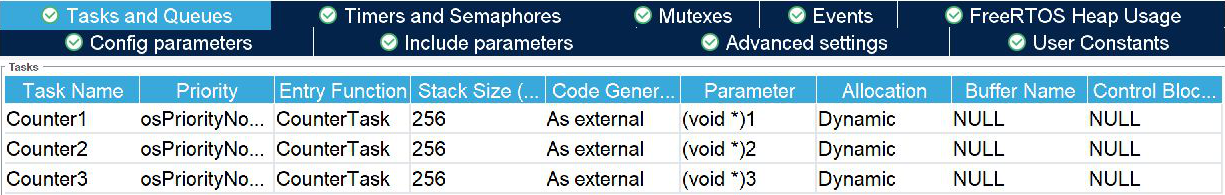
\includegraphics[width=\textwidth]{figures/cubemx_tasks.png}
\caption{The three counter tasks share an entry function and receive distinct identifiers.}
\label{fig:configuration}
\end{figure}

\subsection{Counter Behaviour}
Starting from zero, each successful critical section adds one to the shared counter. Thus, after $N$ successful updates, the counter is $N$ and the printed values follow $1,2,\ldots,N$. Figure~\ref{fig:mutex} contrasts a possible lost update with serialised access. The scheduler determines which task acquires the mutex; the displayed task identifiers follow that acquisition order.

\begin{figure}[H]
\centering
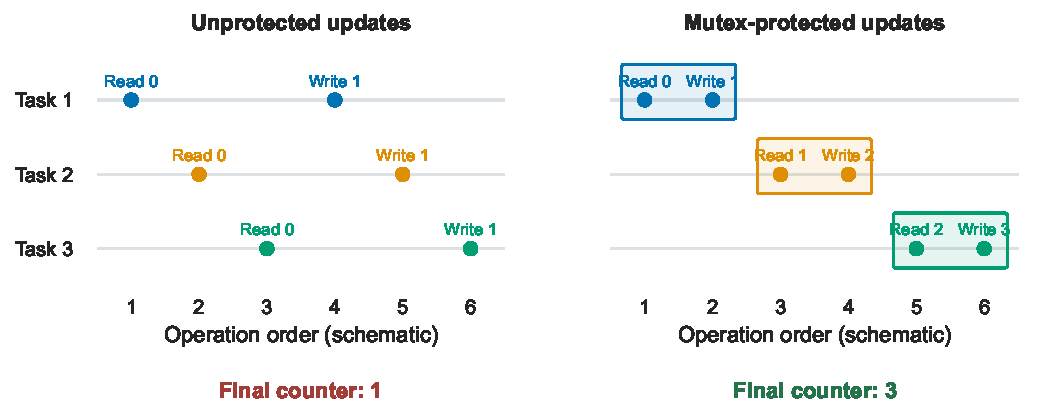
\includegraphics[width=0.95\textwidth]{figures/mutex_interleaving.pdf}
\caption{Illustrative operation order for three increments. Without protection, three reads of zero can produce three writes of one. With the mutex, each task reads the preceding task's updated value.}
\label{fig:mutex}
\end{figure}

\clearpage
\subsection{Commented Implementation}
Initialisation creates the shared mutex and three tasks with distinct identifiers before starting the scheduler (Listing~\ref{lst:creation}).

\begin{lstlisting}[caption={Creation of the mutex and three tasks.},label={lst:creation}]
osKernelInitialize();
/* Create the shared lock before any counter task can run. */
counterMutexHandle = osMutexNew(&counterMutex_attributes);
/* Pass a different identifier to each instance of CounterTask. */
Counter1Handle = osThreadNew(CounterTask, (void *)1, &Counter1_attributes);
Counter2Handle = osThreadNew(CounterTask, (void *)2, &Counter2_attributes);
Counter3Handle = osThreadNew(CounterTask, (void *)3, &Counter3_attributes);
osKernelStart();
\end{lstlisting}

Listing~\ref{lst:counter} implements all three tasks. Each iteration attempts to acquire the mutex with a timeout of zero. A successful acquisition permits one counter increment and one UART message, followed by release of the mutex. If the mutex is occupied, that iteration skips the update. Every iteration ends with a delay of 1000 ticks, corresponding to 1 s at the configured tick rate.

\lstinputlisting[caption={The shared counter task and its critical section.},label={lst:counter}]{../Firmware/Lab4/Lab4/Src/task1.c}

The UART helper in Listing~\ref{lst:console} prints the task identifier and updated count. Transmission remains inside the mutex-protected section, so the counter update and its complete message are ordered together. For example, \texttt{Task 2: 7} denotes the seventh successful increment, performed by task 2.

\lstinputlisting[caption={UART output for a successful counter update.},label={lst:console}]{../Firmware/Lab4/Lab4/Src/console.c}

\clearpage
\section{Task 2: Mutexes and Semaphores}
A mutex grants exclusive ownership of a shared resource to one task. A semaphore maintains a token count: acquisition consumes a token, and release supplies a token. Binary semaphores have a maximum count of one; counting semaphores can represent several available resources (Table~\ref{tab:comparison}).

\begin{table}[H]
\centering
\caption{Mutex and semaphore properties in CMSIS-RTOS2 with FreeRTOS.}
\label{tab:comparison}
\small
\renewcommand{\arraystretch}{1.05}
\begin{tabularx}{\textwidth}{@{}>{\raggedright\arraybackslash}p{27mm}>{\raggedright\arraybackslash}X>{\raggedright\arraybackslash}X@{}}
\toprule
Property & Mutex & Semaphore \\
\midrule
Purpose & Protect a shared resource or critical section & Signal an event or count available resources \\
State & Unlocked, or locked by one owner & Token count from zero to the configured maximum \\
Ownership & The acquiring task owns the mutex & Tokens have no task ownership \\
Release & Performed by the owning task & May be performed by another task or an interrupt service routine \\
Priority inheritance & Raises the owner's priority when a higher-priority task waits & Not provided by binary or counting semaphores \\
Interrupt use & Acquisition and release operate in task context & Release can signal an event from an interrupt \\
\bottomrule
\end{tabularx}
\end{table}

\subsection{Application: UART Receive Completion}
A binary semaphore can notify a worker task when a UART frame has arrived. The semaphore is created with a maximum count of one and an initial count of zero. The worker calls \texttt{osSemaphoreAcquire(completion, osWaitForever)} and blocks while it waits for the frame.

\begin{figure}[H]
\centering
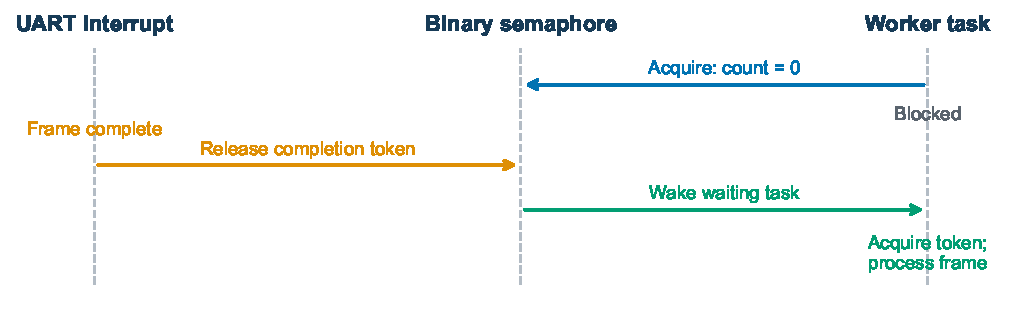
\includegraphics[width=0.92\textwidth]{figures/semaphore_handoff.pdf}
\caption{UART completion signalling with a binary semaphore.}
\label{fig:semaphore}
\end{figure}

When reception completes, the UART callback calls \texttt{osSemaphoreRelease(completion)}. The worker becomes ready, acquires the token when scheduled, processes the received frame, and rearms reception. Figure~\ref{fig:semaphore} shows this sequence. The interrupt performs the notification, while the task performs the frame processing.

A mutex cannot provide this handover: the interrupt is not the owning task, and mutex acquisition and release are unavailable in interrupt context. The semaphore directly represents completion of the receive operation and permits the interrupt to notify the waiting task.

\section{Conclusion}
The three-task application uses one mutex to serialise counter updates and their UART messages, preserving one increment per successful acquisition. Mutex ownership protects shared state, while semaphore tokens support event signalling and resource counting. UART receive completion illustrates how a semaphore connects an interrupt to subsequent task processing.

\end{document}
